\chapter{Конструкторская часть}

В данном разделе будут представлены схемы алгоритмов сортировки: алгоритма битонной сортировки, алгоритма поразрядной сортировки и алгоритма сортировки пузырьком.
. 
\section{Разработка алгоритмов}

На рисунке \ref{img:bitonic_sort_1} -- \ref{img:bitonic_sort_2} приведена схема алгоритма битонной сортировки. 
Схема алгоритма поразрядной сортировки приведена на рисунках \ref{img:radix_sort_1} -- \ref{img:radix_sort_3}, схема алгоритма сортировки пузырьком приведена на рисунках \ref{img:bubble_sort}.

\begin{figure}[h]
	\begin{center}
		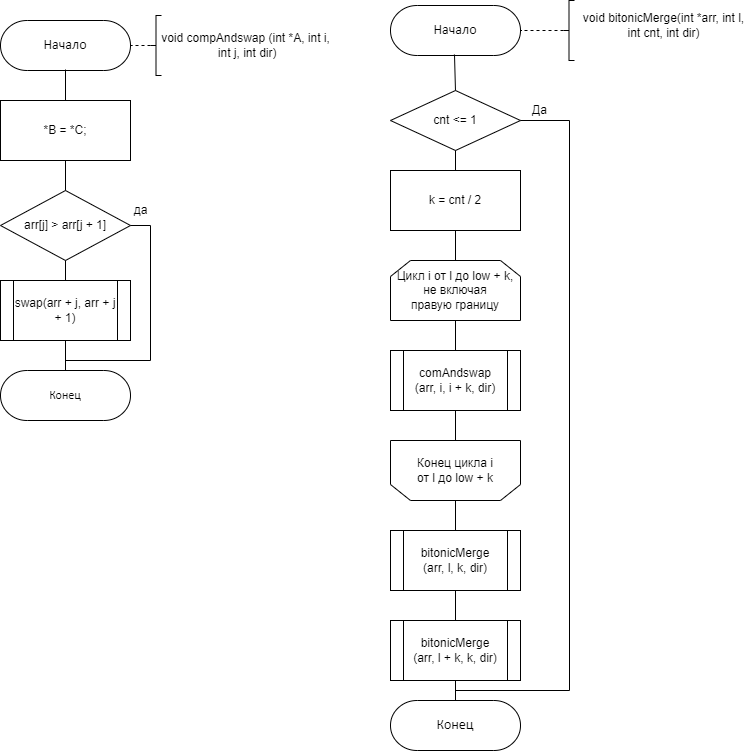
\includegraphics[scale=0.6]{img/bitonic_sort_1.png}
	\end{center}
	\captionsetup{justification=centering}
	\caption{Aлгоритм битонной сортировки}
	\label{img:bitonic_sort_1}
\end{figure}
\clearpage
\begin{figure}[h]
	\begin{center}
		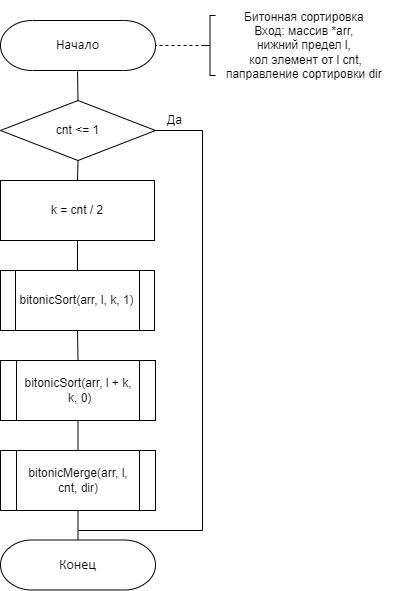
\includegraphics[scale=0.7]{img/bitonic_sort_2.png}
	\end{center}
	\captionsetup{justification=centering}
	\caption{Aлгоритм битонной сортировки (продолжение)}
	\label{img:bitonic_sort_2}
\end{figure}
\clearpage
\begin{figure}[h]
	\begin{center}
		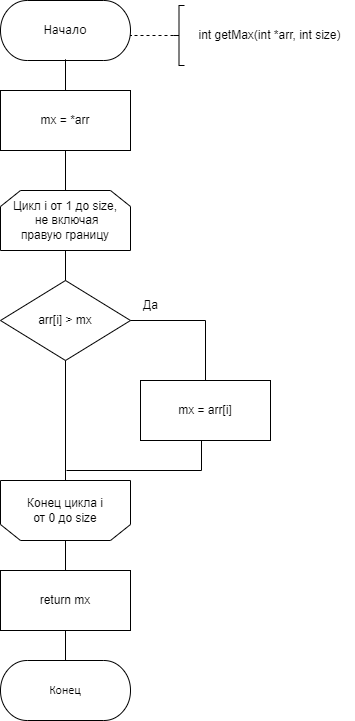
\includegraphics[scale=0.7]{img/radix_sort_1.png}
	\end{center}
	\captionsetup{justification=centering}
	\caption{Aлгоритм поразрядной сортировки}
	\label{img:radix_sort_1}
\end{figure}
\clearpage
\begin{figure}[h]
	\begin{center}
		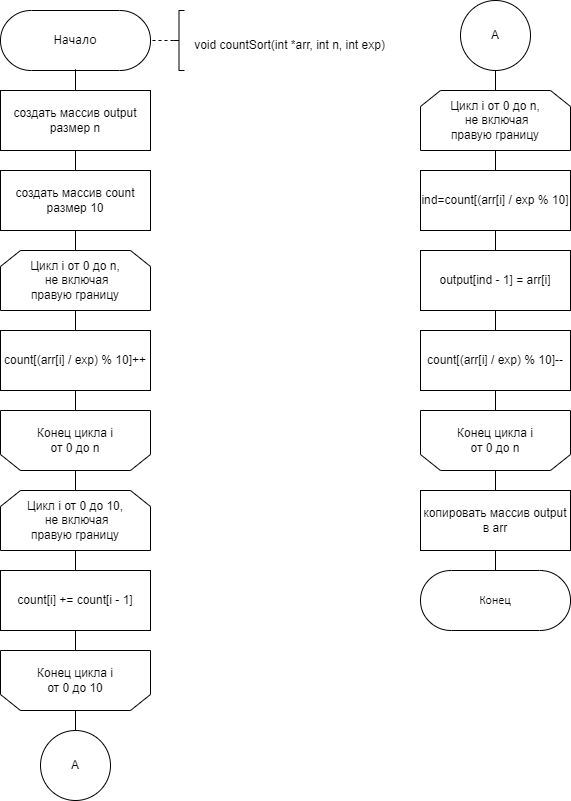
\includegraphics[scale=0.7]{img/radix_sort_2.png}
	\end{center}
	\captionsetup{justification=centering}
	\caption{Aлгоритм поразрядной сортировки (продолжение)}
	\label{img:radix_sort_2}
\end{figure}
\clearpage
\begin{figure}[h]
	\begin{center}
		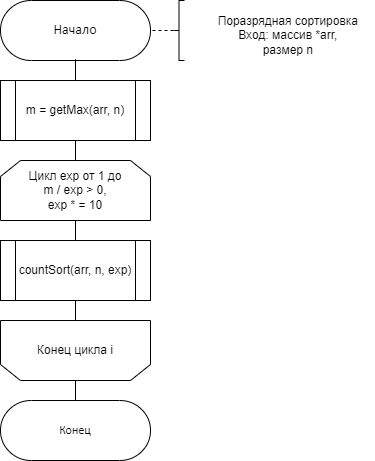
\includegraphics[scale=0.7]{img/radix_sort_3.png}
	\end{center}
	\captionsetup{justification=centering}
	\caption{Aлгоритм поразрядной сортировки (продолжение)}
	\label{img:radix_sort_3}
\end{figure}
\clearpage
\begin{figure}[h]
	\begin{center}
		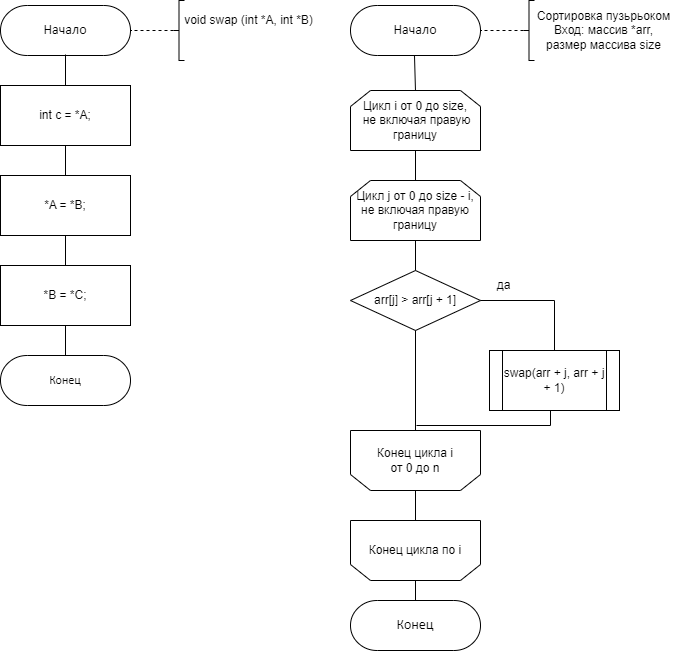
\includegraphics[scale=0.7]{img/bubble_sort.png}
	\end{center}
	\captionsetup{justification=centering}
	\caption{Aлгоритма сортировки пузырьком}
	\label{img:bubble_sort}
\end{figure}
\clearpage

\section{Модель вычислений для оценки трудоемкости алгоритмов}

Для определения трудоемкости алгоритмов необходимо ввести модель вычислений \cite{alg1}:

\begin{enumerate}
	\item операции из списка (\ref{for:operation1}) имеют трудоемкость равную 2;
	\begin{equation}
		\label{for:operation1}
		*, /, \%, *=, /=, \%=
	\end{equation}
	\item операции из списка (\ref{for:operations2}) имеют трудоемкость равную 1;
	\begin{equation}
		\label{for:operations2}
		+, -, +=, -=, =, ==, !=, <, >, <=, >=, [], ++, {-}-
	\end{equation}
	\item трудоемкость оператора выбора \code{if условие then A else B} рассчитывается, как (\ref{for:if});
	\begin{equation}
		\label{for:if}
		f_{if} = f_{\text{условия}} +
		\begin{cases}
			f_A, & \text{если условие выполняется,}\\
			f_B, & \text{иначе.}
		\end{cases}
	\end{equation}
	\item трудоемкость цикла рассчитывается, как (\ref{for:cycle});
	\begin{equation}
		\label{for:cycle}
		f_{for} = f_{\text{инициализации}} + f_{\text{сравнения}} + N(f_{\text{тела}} + f_{\text{инкремент}} + f_{\text{сравнения}})
	\end{equation}
	\item трудоемкость вызова функции равна 0.
\end{enumerate}
\clearpage
\section{Трудоемкость алгоритмов}

Проведем сравнительный анализ реализованных алгоритмов по трудоемкости для сортировки массивы
arr[N].

\subsection{Aлгоритм битонной сортировки}

Трудоемкость данного алгоритма будет складываться из:

\begin{itemize}
	\item трудоемкости процесса создания битонной последовательности равной $\log_{2}N \cdot 3$;
	\item трудоекмости процесса сравнения элементы 2 последовательности равной $\log_{2}N \cdot (3 + 2)$;
\end{itemize}

Таким образом, трудоемкость стандартного алгоритма умножения равна:
\begin{equation}
	\label{for:radix}
	f = \log_{2}N \cdot 3 * (\log_{2}N \cdot (3 + 2)) = O(log^2 N)
\end{equation}
\subsection{Aлгоритм поразрядной сортировки}

Трудоемкость данного алгоритма будет складываться из:

\begin{itemize}
	\item трудоемкости определения максимальное значение массива равной $2 + 3 \cdot N$;
	\item трудоемкости определения сортированный массив по каждому разряду равной
	 $2 + N\cdot 8 + 2 + 10 \cdot 4 + 3 + N \cdot 17 = 47 + 25N$;
	\item трудоемкости главного цикла равной $2 + log_{10} M \cdot (47 + 25N)$;
\end{itemize}

Трудоемкость алгоритма поразрядной сортировки, где M --- максимальное значение массива, равна:
\begin{equation}
	\label{for:radix}
	f = 2 + 3 \cdot N + 2 + log_{10}M\cdot(47 + 25N) \approx 25N\cdot\log_{10}M = O(N\log{M})
\end{equation}

\subsection{Aлгоритма сортировки пузырьком}

Трудоемкость в лучшем случае при отсортированном массиве, когда ничего не обменивается, но все же данные рассматриваются. 
Трудоемкость алгоритма в лучшем случае равна:

\begin{equation}
	\label{for:bubble1}
	f_{best} =  2 + N \cdot(2 + 4 \cdot N) \approx O(N ^ 2)
\end{equation}
Трудоемкость в худшем случае при отсортированном массиве, когда массиве в обратном порядке. Трудоемкость алгоритма в худшем случае равна:
\begin{equation}
	\label{for:bubble2}
	f_{worst} =  2 + N \cdot(2 + 14 \cdot N) \approx O(N ^ 2)
\end{equation}

\section{Вывод}
Были представлены схемы алгоритмов умножения матриц.
Проведённая теоретическая оценка трудоемкости алгоритмов показала, что в трудоёмкость выполнения алгоритма поразрядной сортировки зависит от количество элементов и максимального значения массива.
Тажке трудоёмкость выполнения алгоритма сортировки пузырьком $O(N ^ 2)$ больше чем трудоёмкость выполнения алгоритма битонной сортировки $O(log^2 N)$.